\chapter[Introduction]{Introduction}\label{chap_intro}

%%% REVISAR
The majority of real-world phenomena are spatio-temporal, for example the traffic flow, epidemiological analysis, the diffusion of air pollutants and the regional rainfall. Successfully predicting the future of these spatio-temporal systems based on the past observations is essential for a wide range of scientific studies and real-life applications like traffic management, precipitation nowcasting, and typhoon alert systems.


\section{Motivation}
\label{Sec:Motivation}

Recent works \cite{Ghanta022019, Crankshaw2017, Polyzotis2018}, highlight some challenges found in spatio-temporal predictive serving systems. In such systems, values of variables whose behavior varies in space-time are inferred by predictive models built over regions of the spatio-temporal domain. In this context, we are interested in the problem arising in the presence of multiple competing predictive models, i.e., models that predict the same variable but are built independently over potentially different regions of the domain. It may be the case in large companies where autonomously developed models about the same phenomenon (a.k.a. competing models) are deployed and used to answer predictive queries. 

A predictive serving system enables users to express queries that specify: a spatio-temporal region, a target variable, and an evaluation metric. The outcome of the query presents the target variable's values on the specified region computed by predictive models that maximize the evaluation metric. 

However, identifying the  models to be used by the system to answer the predictive query is a hard problem. It is due to the fact that competing models present varying predictive behavior throughout regions of the domain. This can be explained by the learners' intrinsic learning capabilities and variations on spatio-temporal regions used to construct independently built models. In this context, we want to define a procedure that selects a set of models to compute the query answer and maximize the evaluation metric. 

\begin{figure}[h]
	\centering
	
\includegraphics[scale=0.31]{../Figures/ModelManagementPS-VersionCompleta}
	\caption{Predictive Serving System Models.}
	\label{Fig:MotiPoster}
	%	\Description{ML Model Lifecycle.}
\end{figure}

In Figure \ref{Fig:MotiPoster}, we show the workflow of a Predictive Serving System; our work is focused mainly on the training phase, but we also consider some aspects of the deployment phase (which is more relevant for machine learning models). To validate our approach in those areas, we implement a very simple prediction service.

%Conversely, in spatio-temporal regions specified by the query and that have not been used for training, the model would exhibit an error computed as a function of the distance between the query non seen data region and the model building data region.

\subsection{Problem Statement}
\label{Sec:ProblemStatement}

Given a phenomenon with a spatio-temporal domain, represented by univariate time series, where independent predictive models have been trained, select a model or a composition of models to answer a spatio-temporal predictive query that maximizes an evaluation metric.

Our approach aims to evaluate the predictive quality of models by characterizing temporal patterns within the predictive variable domain data. In particular, we identify some temporal patterns on domain regions where the models have been trained and compare them against temporal patterns within the query spatio-temporal region. 

An important hypothesis that will be validated in this work is that, if a query region has similar data patterns as the regions used to train the model, then the behavior of the model on the query region should follow the one observed during training.

We argue that it should be preferable to use a partitioning technique that considers grouping domain elements based on the similarity of their temporal evolution, rather than creating groups just according to a regular division of the domain geometry.

\section{Objective and Contribution}
\label{Sec:ObjectiveContribution}

% Objective
The main objective of our work is to develop a methodology that can be used to make predictions about future states of a spatio-temporal region, using carefully selected predictive models that have been trained with limited temporal data, but at the same time produce predictions about unseen temporal data within some tolerated error margin. 

% Contribution
We now highlight some important contributions of this work to the state of the art of the relevant literature:

\begin{itemize}
\item A comprehensive approach for grouping temporal elements based on their shape; this approach can calculate elements that generalize certain regions of the spatio-temporal domain. %A novel approach for model composition in a spatio-temporal domain with high data volume, expressed as a classification problem and supported by a hybrid (machine learning). We validated this approach against a naive baseline and a simpler approach based on a single partitioning scheme. We verified that the solution is viable in an environment for online spatio-temporal predictive queries.



%By understanding the process of the partitioning scheme based on DTW distances, we were able to implement this step efficiently using parallelization and persistence, and therefore gain a considerable reduction in the computational resources and time required to perform the operations. With experimental analysis using another partitioning scheme as a baseline, we were able to verify the robustness of the proposed partitioning algorithm.
% To verify this, we compare the intra-cluster sum of both partitioning techniques for several values of $k$.

\item A flexible analysis of the forecast errors produced by predictive models. 
%We successfully applied the same forecast error analysis for the main type of predictive model (ARIMA) and another type of model used as baseline ($k$NN). This same approach can be useful for other types of predictive models and different spatio-temporal problems.

\item A time series classification approach for model selection. 
%A novel approach for model composition in a spatio-temporal domain with high data volume, expressed as a classification problem and supported by a hybrid (machine learning). We validated this approach against a naive baseline and a simpler approach based on a single partitioning scheme. We verified that the solution is viable in an environment for online spatio-temporal predictive queries.
\end{itemize}

%%% GINO REVISAR
Considering the computational aspects of the problem proposed, we include a technical contribution in the form of a tool that allow us to develop our methodology, an open-source Python package designed to work with spatio-temporal data and predictive models. This tool support the steps in the workflow showed in Figure \ref{Fig:MotiPoster}, and also the implementation of experiments to evaluate and analyze several aspects of the methodology.

% \begin{itemize}
% \item An open-source Python package designed to work with spatio-temporal data and predictive models. 
%This package was developed to implement a computational solution to execute the methodology described in this work. However, it can be easily adapted and extended for other similar purposes in the field of spatio-temporal analysis.
%  \end{itemize}
 
These contributions stem from the proposed methodology and its evaluation, and will be elaborated further during the next few chapters and revisited in the conclusion of this work.

\section{Problem Formalization}
\label{Sec:ProblemFormalization}

%% GINO REVISAR
This formalization enables us to adequately and consistently describe the different processes and components involved in the proposed methodology and corresponding flow of data. The axes $\left(T, X, Y\right)$ represent the spatio-temporal dimensions, where $T$ is the temporal axe for the time index, and $(X,Y)$ indicate the spatial position for the variable(s) of interest, as shown in Figure \ref{fig:time-series}.

Let $\mathcal{D} = \{(\mathcal{S},( x, y)): \,\, \mathcal{S} = \{s_{0}, s_{1}, s_{2}, \ldots, s_{t}\}$ denote a univariate time-series in the axe $T$, and $(x,y) \in (X,Y)\}$, represent a spatio-temporal domain. Denote by $\mathcal{G} = \{g_{1}, g_{2}, \ldots \}$ the set of temporal predictive models that were trained for different subsets $\mathbf{S} \subseteq \mathcal{D}$. Each predictive model $g\in \mathcal{G}$ is denoted as follows:

\begin{equation}
\label{eq:ModelDefinition}
g = \langle \mathbf{S}, A, \mathbf{p}, E, \varSigma \rangle,
\end{equation}
where:
\begin{itemize}[noitemsep,nolistsep]	
	\item $\mathbf{S}$: input dataset included in the spatio-temporal domain $\mathcal{D}$,
	\item $A$: learner or hypothesis set,
	\item $\mathbf{p}$: model parameters (number of time-units to obtain the in-sample error ($t_{p}$), number of time-units to forecast ($t_{f}$)),
	% REVIEW !!!
	\item $E$: in-sample error (generally computed by the difference between the predicted value by $g$ and the actual value in the dataset),
	\item $\varSigma$: implementation/execution quality metrics.
\end{itemize}
%\noindent In Figure \ref{fig:time-series}, we show the elements involved in the formalization of our problem:
\begin{figure}[htb]
	\centering
	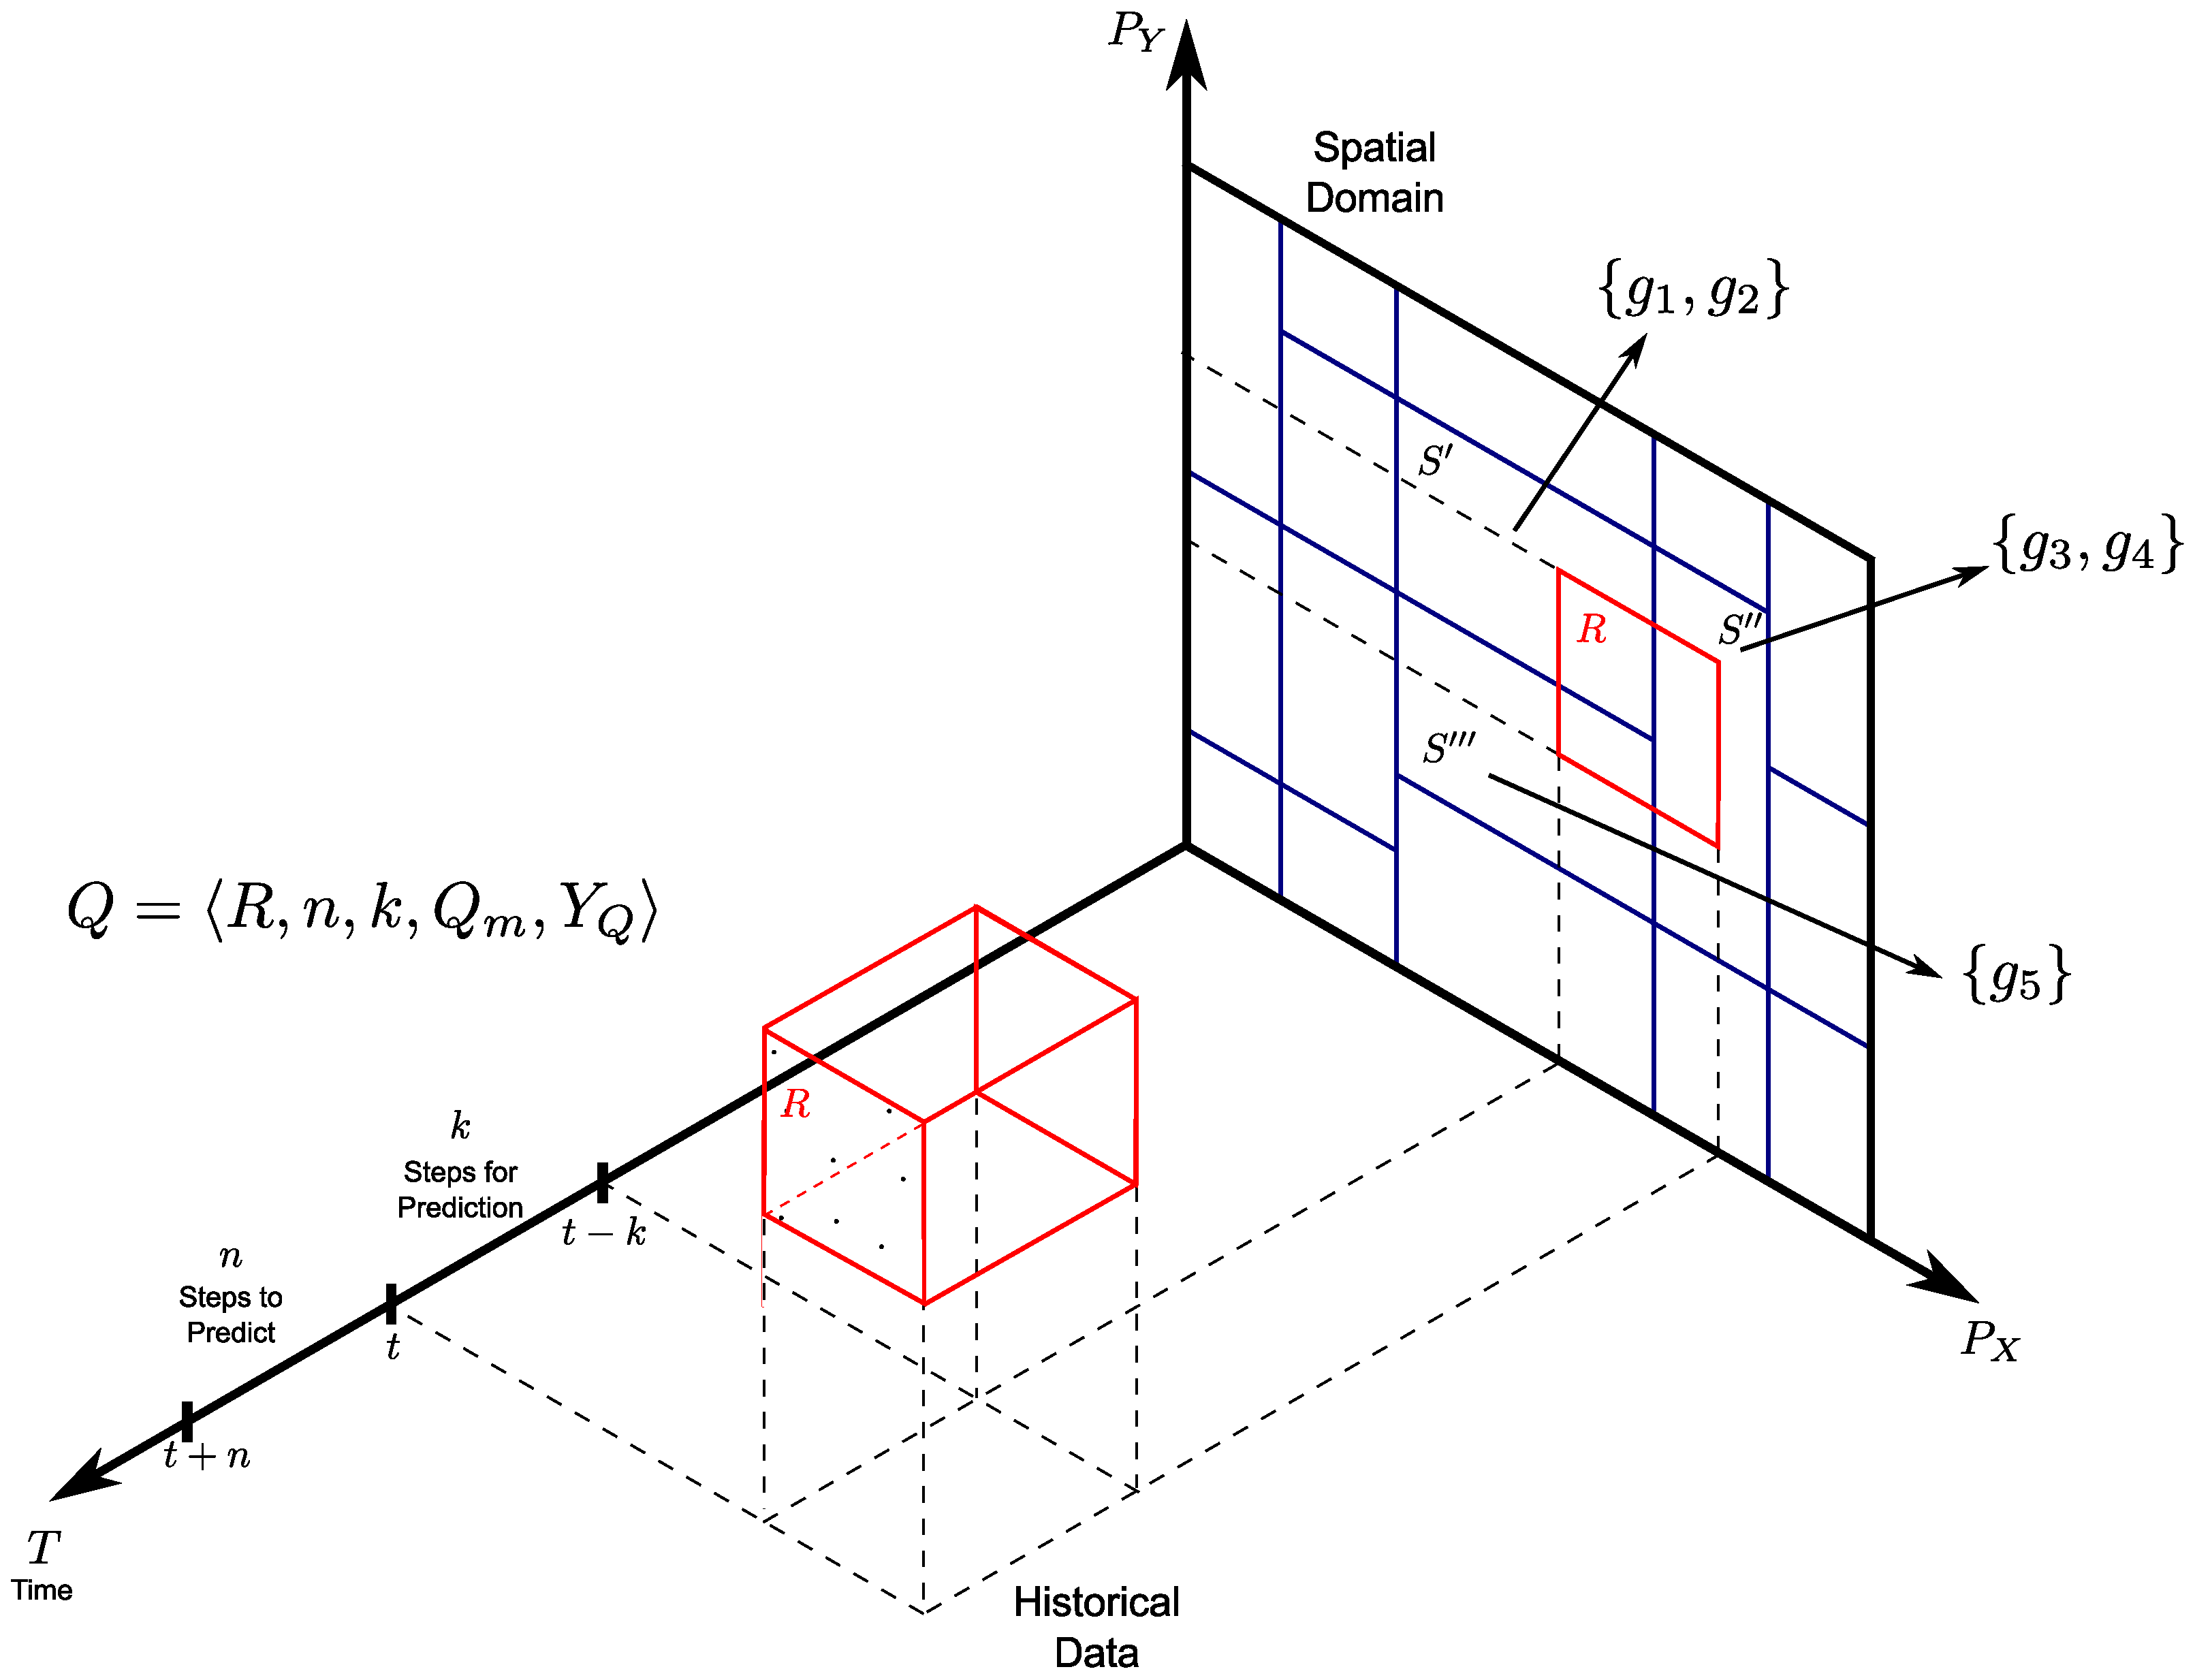
\includegraphics[scale=0.25]{../Figures/RepresentationTimeSeries}
	\caption{Predictive Spatio-Temporal Queries.}
	\label{fig:time-series}
\end{figure}

In this context, given a predictive spatio-temporal query $Q$ denoted as:
\begin{equation} \label{eq:predictivequery}
Q = \langle R, t_{p}, t_{f}, Q_{m} \rangle,
\end{equation}
where:
\begin{itemize}[noitemsep,nolistsep]	
	\item $R$: represents the size/shape/type of interest region,
	\item $t_{p}$: $\{s_{t-t_p}, s_{t-t_{p}+1}\ldots, s_{t}\}$ number of steps used for  prediction,
	\item $t_{f}$: $\{s_{t+1}, \ldots, s_{t+t_f}\}$ number of steps to predict ($n\geq 1$),
	\item $Q_{m}$: represent users quantitative measurements to evaluate the predictive output.
\end{itemize}
We are interested in processing this query using the models $g$ in a way that guarantees a degree of accuracy. We formally define our problem: Let the spatio-temporal domain characterization $\mathcal{D} = \bigcup_{i=1}^{n} \mathbf{S_i}$ and $\mathcal{G}$ the set of temporal models for a single element of $\mathbf{S_i}$ that accounts for the in-sample error bounds for the elements in $\mathbf{S_i}$. Given $Q = \langle R, t_{p}, t_{f}, Q_{m} \rangle$:

\begin{equation}
\textrm{For all}\, \mathcal{S} \in R: \textrm{Find a\, } g \in \mathcal{G'} \,\,\textrm{such that} \,\, \argminA_{g\in\mathcal{G'}} E_{g}(R).
\end{equation}

%TODO Change the argmin 


\section{Thesis Outline}
\label{Sec:ThesisOutline}

The structure of the remainder of this thesis is outlined for reference.

\begin{description}
\item[Chapter 2.] \textbf{[Theoretical Foundations.]} Presents the fundamental approaches of methods and techniques for the task of univariate time series clustering, using shape-based similarity in particular. It is followed by the foundations of neural network approaches for the task of univariate time series classification. Finally, we consider the foundations for time series analysis, with a focus on auto-regressive methods.

\item[Chapter 3.] \textbf{[Related Works.]} Covers a review of other works found in the literature that use similar methods and techniques utilized in our proposed methodology. We include some comparisons that help put our work into context. 

\item[Chapter 4.] \textbf{[Methodology.]} This chapter is dedicated to elaborating the methodology proposed in this work, providing justifications for some decisions made and establishing hypotheses that can be later validated via experiments.

%\item[Chapter 5.] \textbf{[Spatio Temporal Tool for Time Series Analysis.]} Describes some architectural aspects of an application designed to implement the proposed methodology and perform the experiments to validate our proposal.

\item[Chapter 5.] \textbf{[Experimental Results.]} Describes the experimental evaluation of the methodology, considering a case study of temperature forecasting. The experiments are organized according to the steps considered in the methodology; for each step, we perform extensive analyses and discuss the results obtained. 

\item[Chapter 6.] \textbf{[Conclusions and Future Works.]} Finally, in this chapter, the main contributions of the thesis are highlighted, and we indicate some future directions for research based on this work.

\end{description}

Additionally, in the Appendix we include some architectural aspects of an application called `Spatio-Temporal Tool for Time-Series Analysis', designed to implement the proposed methodology and perform the experiments to evaluate our proposal.